\documentclass[11pt,a4paper]{article}
\usepackage[T1]{fontenc}
\usepackage{isabelle,isabellesym}
\usepackage{amssymb}
\usepackage[english]{babel}
\usepackage[only,bigsqcap]{stmaryrd}
\usepackage{eufrak}
\usepackage{textcomp}

% this should be the last package used
\usepackage{pdfsetup}

% urls in roman style, theory text in math-similar italics
\urlstyle{rm}

% for rule output in LaTeXsugar
\usepackage{mathpartir}
\usepackage{graphicx}
\isabellestyle{it}

% this should be the last package used
\usepackage{pdfsetup}

\renewcommand{\isasymacute}{\isatext{\'\relax\hspace{-0.20em}}}
\DeclareRobustCommand{\isactrlesup}{\egroup\egroup\endmath\egroup\relax\hspace{-0.15em}}

\begin{document}

\title{--- \textbf{Simpl} --- \\
       A Sequential Imperative Programming Language\\
       Syntax, Semantics, Hoare Logics and Verification Environment}
\author{Norbert W. Schirmer}

\begin{abstract}
We present the theory of Simpl, a sequential imperative programming language.
We introduce its syntax, its semantics (big and small-step operational
semantics) and Hoare logics for both partial as well as total correctness.
We prove soundness and completeness of the Hoare logic. We
integrate and automate the Hoare logic in Isabelle/HOL to obtain a
practically usable verification environment for imperative programs.

Simpl is independent of a concrete programming language but expressive
enough to cover all common language features: mutually recursive
procedures, abrupt termination and exceptions, runtime faults, local
and global variables, pointers and heap, expressions with side
effects, pointers to procedures, partial application and closures,
dynamic method invocation and also unbounded nondeterminism.
\end{abstract}

\maketitle

\tableofcontents
\parindent 0pt\parskip 0.5ex

\pagebreak

\begin{center}
  \makebox[0pt]{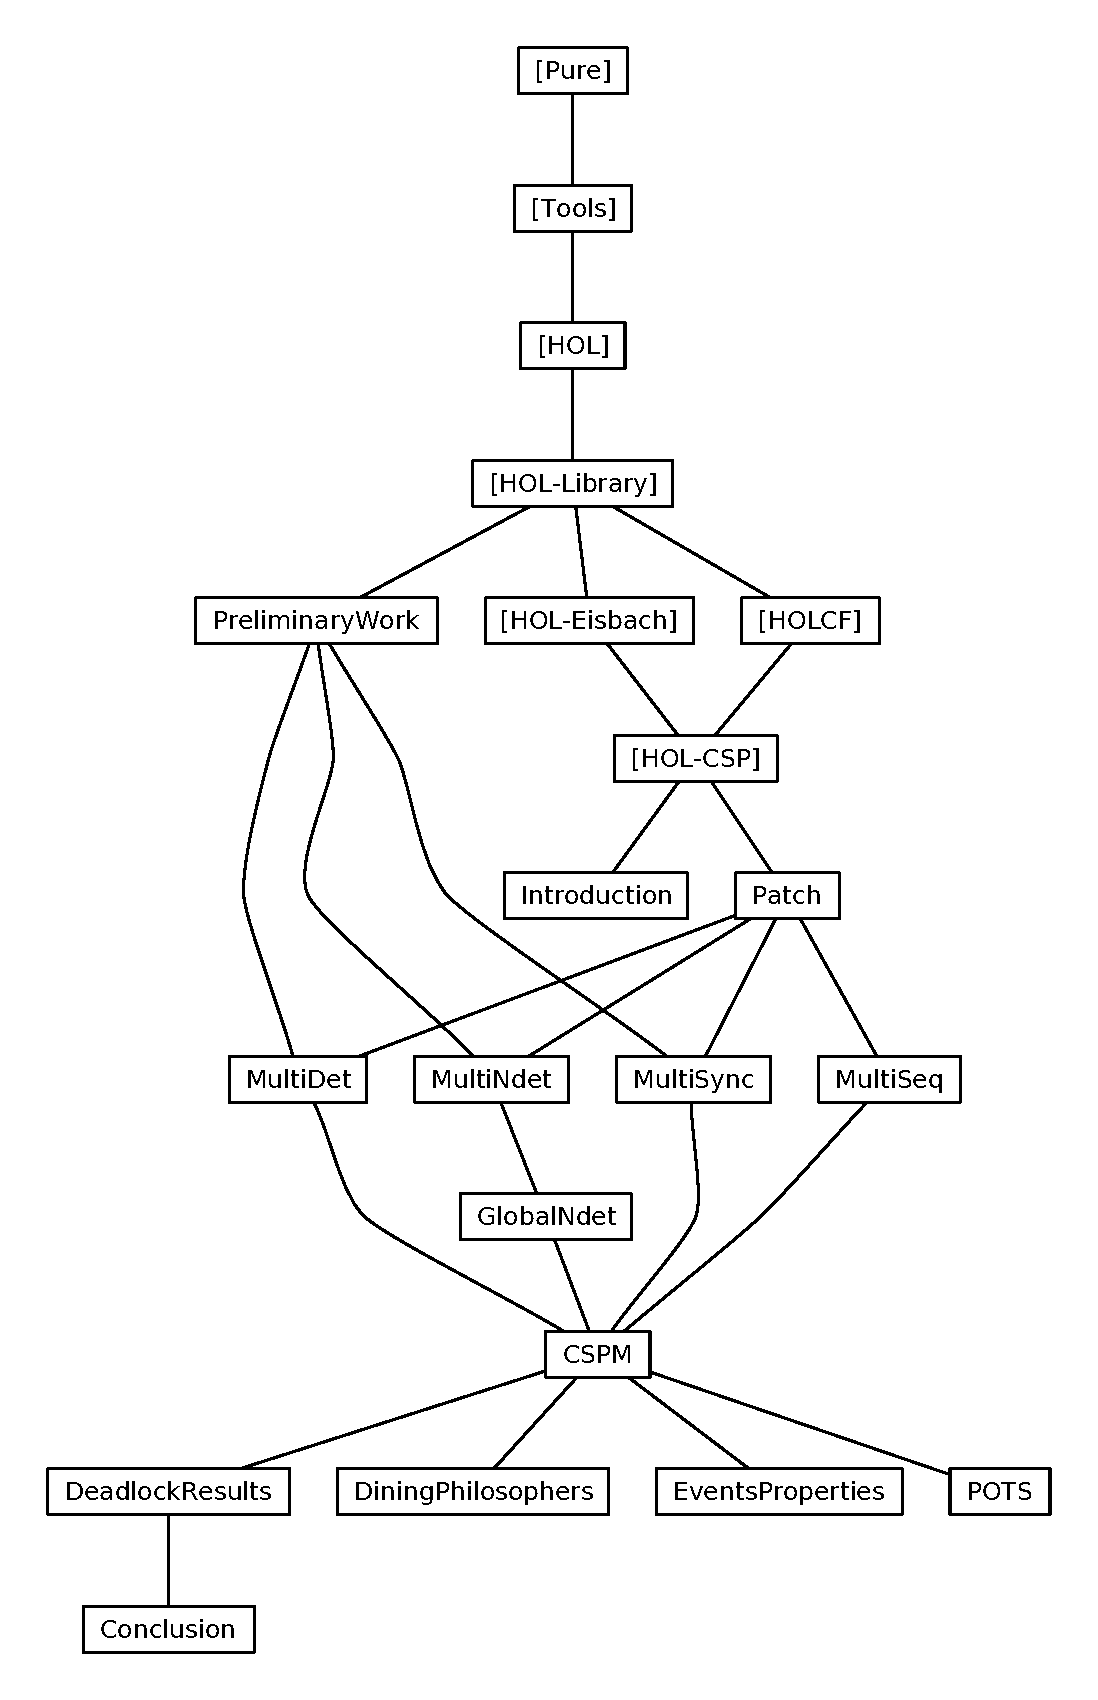
\includegraphics[width=\paperwidth=\textheight,keepaspectratio]{session_graph}
}\end{center}

\pagebreak

\section{Introduction}

The work presented in these theories was developed within the German Verisoft
project\footnote{\url{http://www.verisoft.de}}. A thorough description of the core
parts can be found in my PhD thesis~\cite{Schirmer-PhD}. A tutorial-like user guide
is in Section~\ref{sec:UserGuide}.

Applications so far include BDD-normalisation~\cite{Ortner-Schirmer-TPHOL05},
a C0 compiler~\cite{Leinenbach:SSV08-??}, a page fault handler~\cite{Alkassar:TACAS08-??}
and extensions towards separation logic~\cite{Tuch:separation-logic:2007}.


% generated text of all theories
\input{session}

% optional bibliography
\bibliographystyle{abbrv}
\bibliography{root}

\end{document}

%%% Local Variables:
%%% mode: latex
%%% TeX-master: t
%%% End:
